\section{Background}

``Certain kind of parallel lines are supposed to start converging in such a way that an `end' can be projected by the reader somewhere beyond the right frame. If no such convergence or projection occured to you, then the book's failed for you.'' -- David Foster Wallace \cite{badger_internet_1996}

\subsection{The structure of \infinitejest}

\infinitejest's structure differs from that of a typical book in a number of ways.

\subsubsection{Chronology}

The story is made up of 192 sections which are ordered non-chronologically; as seen in figure~\ref{chronology_bars}, the first sections to occur in the book appear last chronologically.

\begin{figure}[ht]
    \centering
    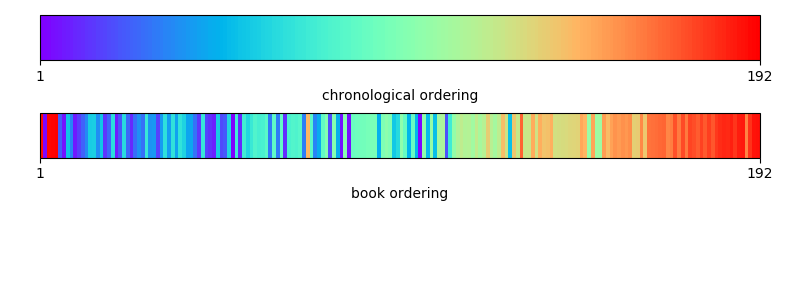
\includegraphics[width=.5\textwidth]{../data/plots/section_bars.png}
    \caption{Contrasting the ordering of events per the book with the chronology presented in \cite{carlisle_2007}}
    \label{chronology_bars}
\end{figure}

\subsubsection{Sierpinski Gasket}

The book's structure is ostensibly based on a Sierpinski Gasket, a triangular fractal.

\begin{figure}[ht]
    \centering
    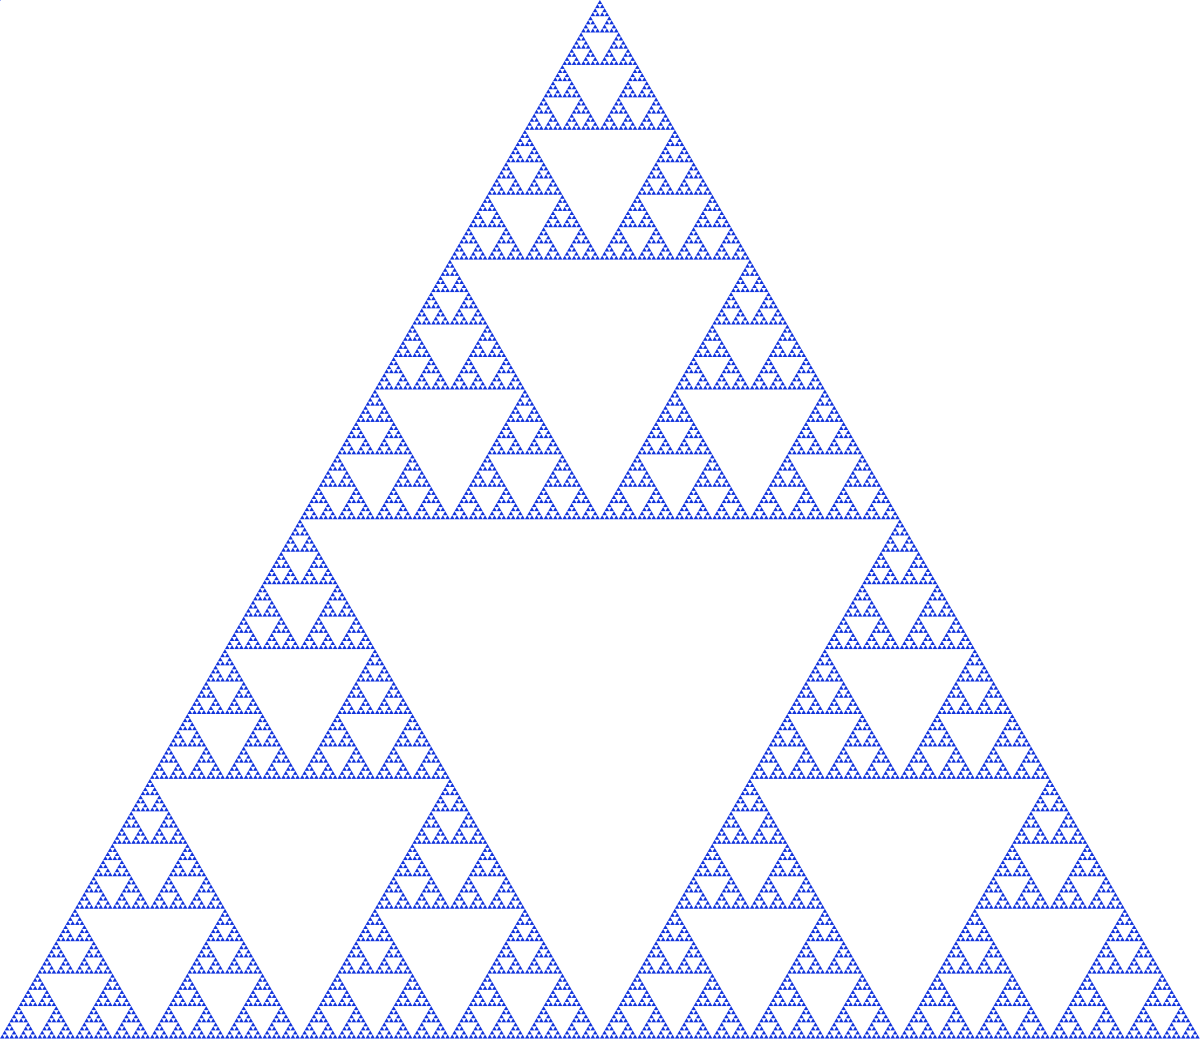
\includegraphics[width=.25\textwidth]{images/sierpinski.png}
    \caption{Sierpinski Gasket}
    \label{Sierpinski Gasket}
\end{figure}

\subsubsection{Endnotes}

The book uses endnotes extensively to convey additional information of varying degrees of relevance. The gamut of information can run from multi-page mini-stories containing important narrative information (\infinitejest, endnote 304) to ``No clue.'' (\infinitejest, endnote 216). Endnotes can reference other endnotes (\infinitejest, endnote 45), and can themselves have endnotes (\infinitejest, endnotes 388). These present a challenge both for the reader and for our approach to generating the network.

\subsection{Related Work}

We are not the first to mine networks from literature or to apply data-driven techniques to evaluate a hypothesis.

Reagan et al.\ use NLP and sentiment to analyze 1,327 stories from Project Gutenberg in an effort to confirm Kurt Vonnegut's rejected Master's thesis categorizing story arcs into six types by emotion; they indeed find six core emotional trajectories, and they use the number of downloads of stories with each archetypal arc-type to evaluate each type's popularity~\cite{Reagan2016}.

Alberich et al. (2002) build bipartite social network out of Marvel comic book character appearances in comic books, finding many similar characteristics to real-life scientific collaboration networks such as short distances and a power-law degree distribution tail with a cutoff~\cite{2002marvel}. Notably, they find a lower clustering coefficient than expected in real networks.

Bonato et al.~\cite{Bonato2016} compared networks for three books: \textit{Twilight}, by Stephanie Meyer, \textit{The Stand} by Steven King, and J.K. Rowling's \textit{Harry Potter and the Goblet of Fire}. They found the Chung-Lu model best fits the co-occurance networks. Game of Thrones and Lord of the Rings have also been similarly analyzed~\cite{GOT,ribeiro2016complex}.

\infinitejest differs from the narratives explored in prior works due its unorthodox narrative structure, the sheer number of characters, and the stylistic diversity of its prose.
